
\chapter{Monte Carlo}
The Monte Carlo method was invented by scientists working on the atomic bomb in the 1940s. Its core idea is to use random samples of parameters or inputs to explore the behavior of a complex system or process.  Nowadays, MC are essential part of both theoretical and experimental particle physics research
This chapter gives an overview of ATLAS experiment simulation scheme, simulation methods and software used. Also, a technique for speeding up this simulation will be discussed. At the end list of the MC samples, used in the analysis will be described
%Also, to avoid statistical fluctuations in MC it is usually required to have 5-10 times more events, than expected in the data.

\section{MC simulation at ATLAS experiment}

\begin{figure}[h]
\center{
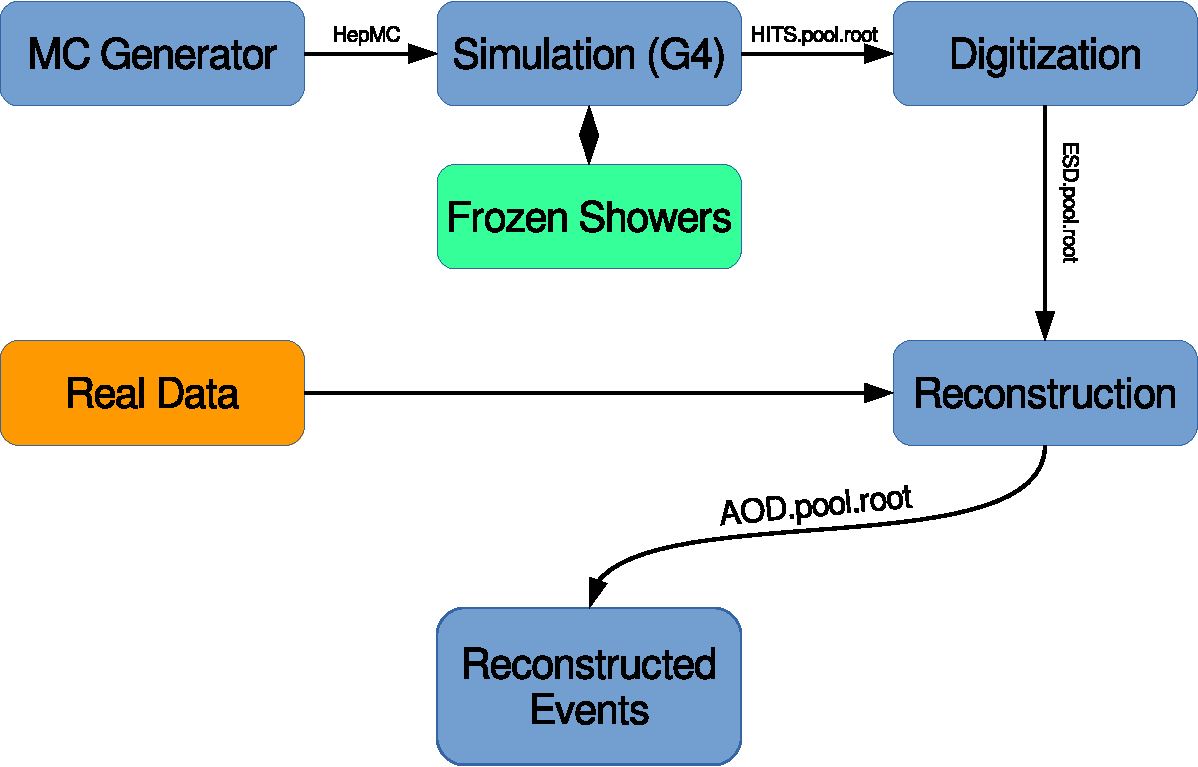
\includegraphics[width=0.6\textwidth]{MC/MC_production_chain2.pdf}
\caption{Diagram of the ATLAS MC production chain}
\label{fig:MC_gen}}
\end{figure}

Monte Carlo is allowing to make different analysis, such as compare data with predictions, study detector or selection algorithms performance. This means, that MC precison is important. Simulation needs to use precise models of physics for sampling and have large enough statistics, to exclude statistical uncertanties (usually 5-10 times more, than expected in a data). ATLAS simulation software is integrated into Athena and usually used during large production of events. Simulation chain is generally divided into 4 main steps (Figure ~\ref{fig:MC_gen}):
\begin{description}
\item[Event generation]Simulation of hard interaction and a resulting high-energy particles parameters. This step is independent of ATLAS detector geometry.
\item[Simulation]Simulation of energy depositions ("hits") done by final state particles in ATLAS detector.
\item[Digitalization] Simulation of detector responce using "hits" information:  first, inputs to the read out drivers (ROD's), called "digits" are constructed, then, ROD functionality is emulated. Detector noise effects are added at this stage. 
\item[Reconstruction] Production of the Analysis Object Data (AOD) files, which are containing sufficient information for physics analysis. This stage is identical for both data and MC
\end{description}
This is scheme is allowing to use computing resources efficiently, than with a single-step simulation, and simplifies software validation, since it is possible to use files from the previous steps with different software version. In the following sections event generation and simulation will be described more detailed

\subsection{Event generators}

\begin{figure}[h]
\begin{center}
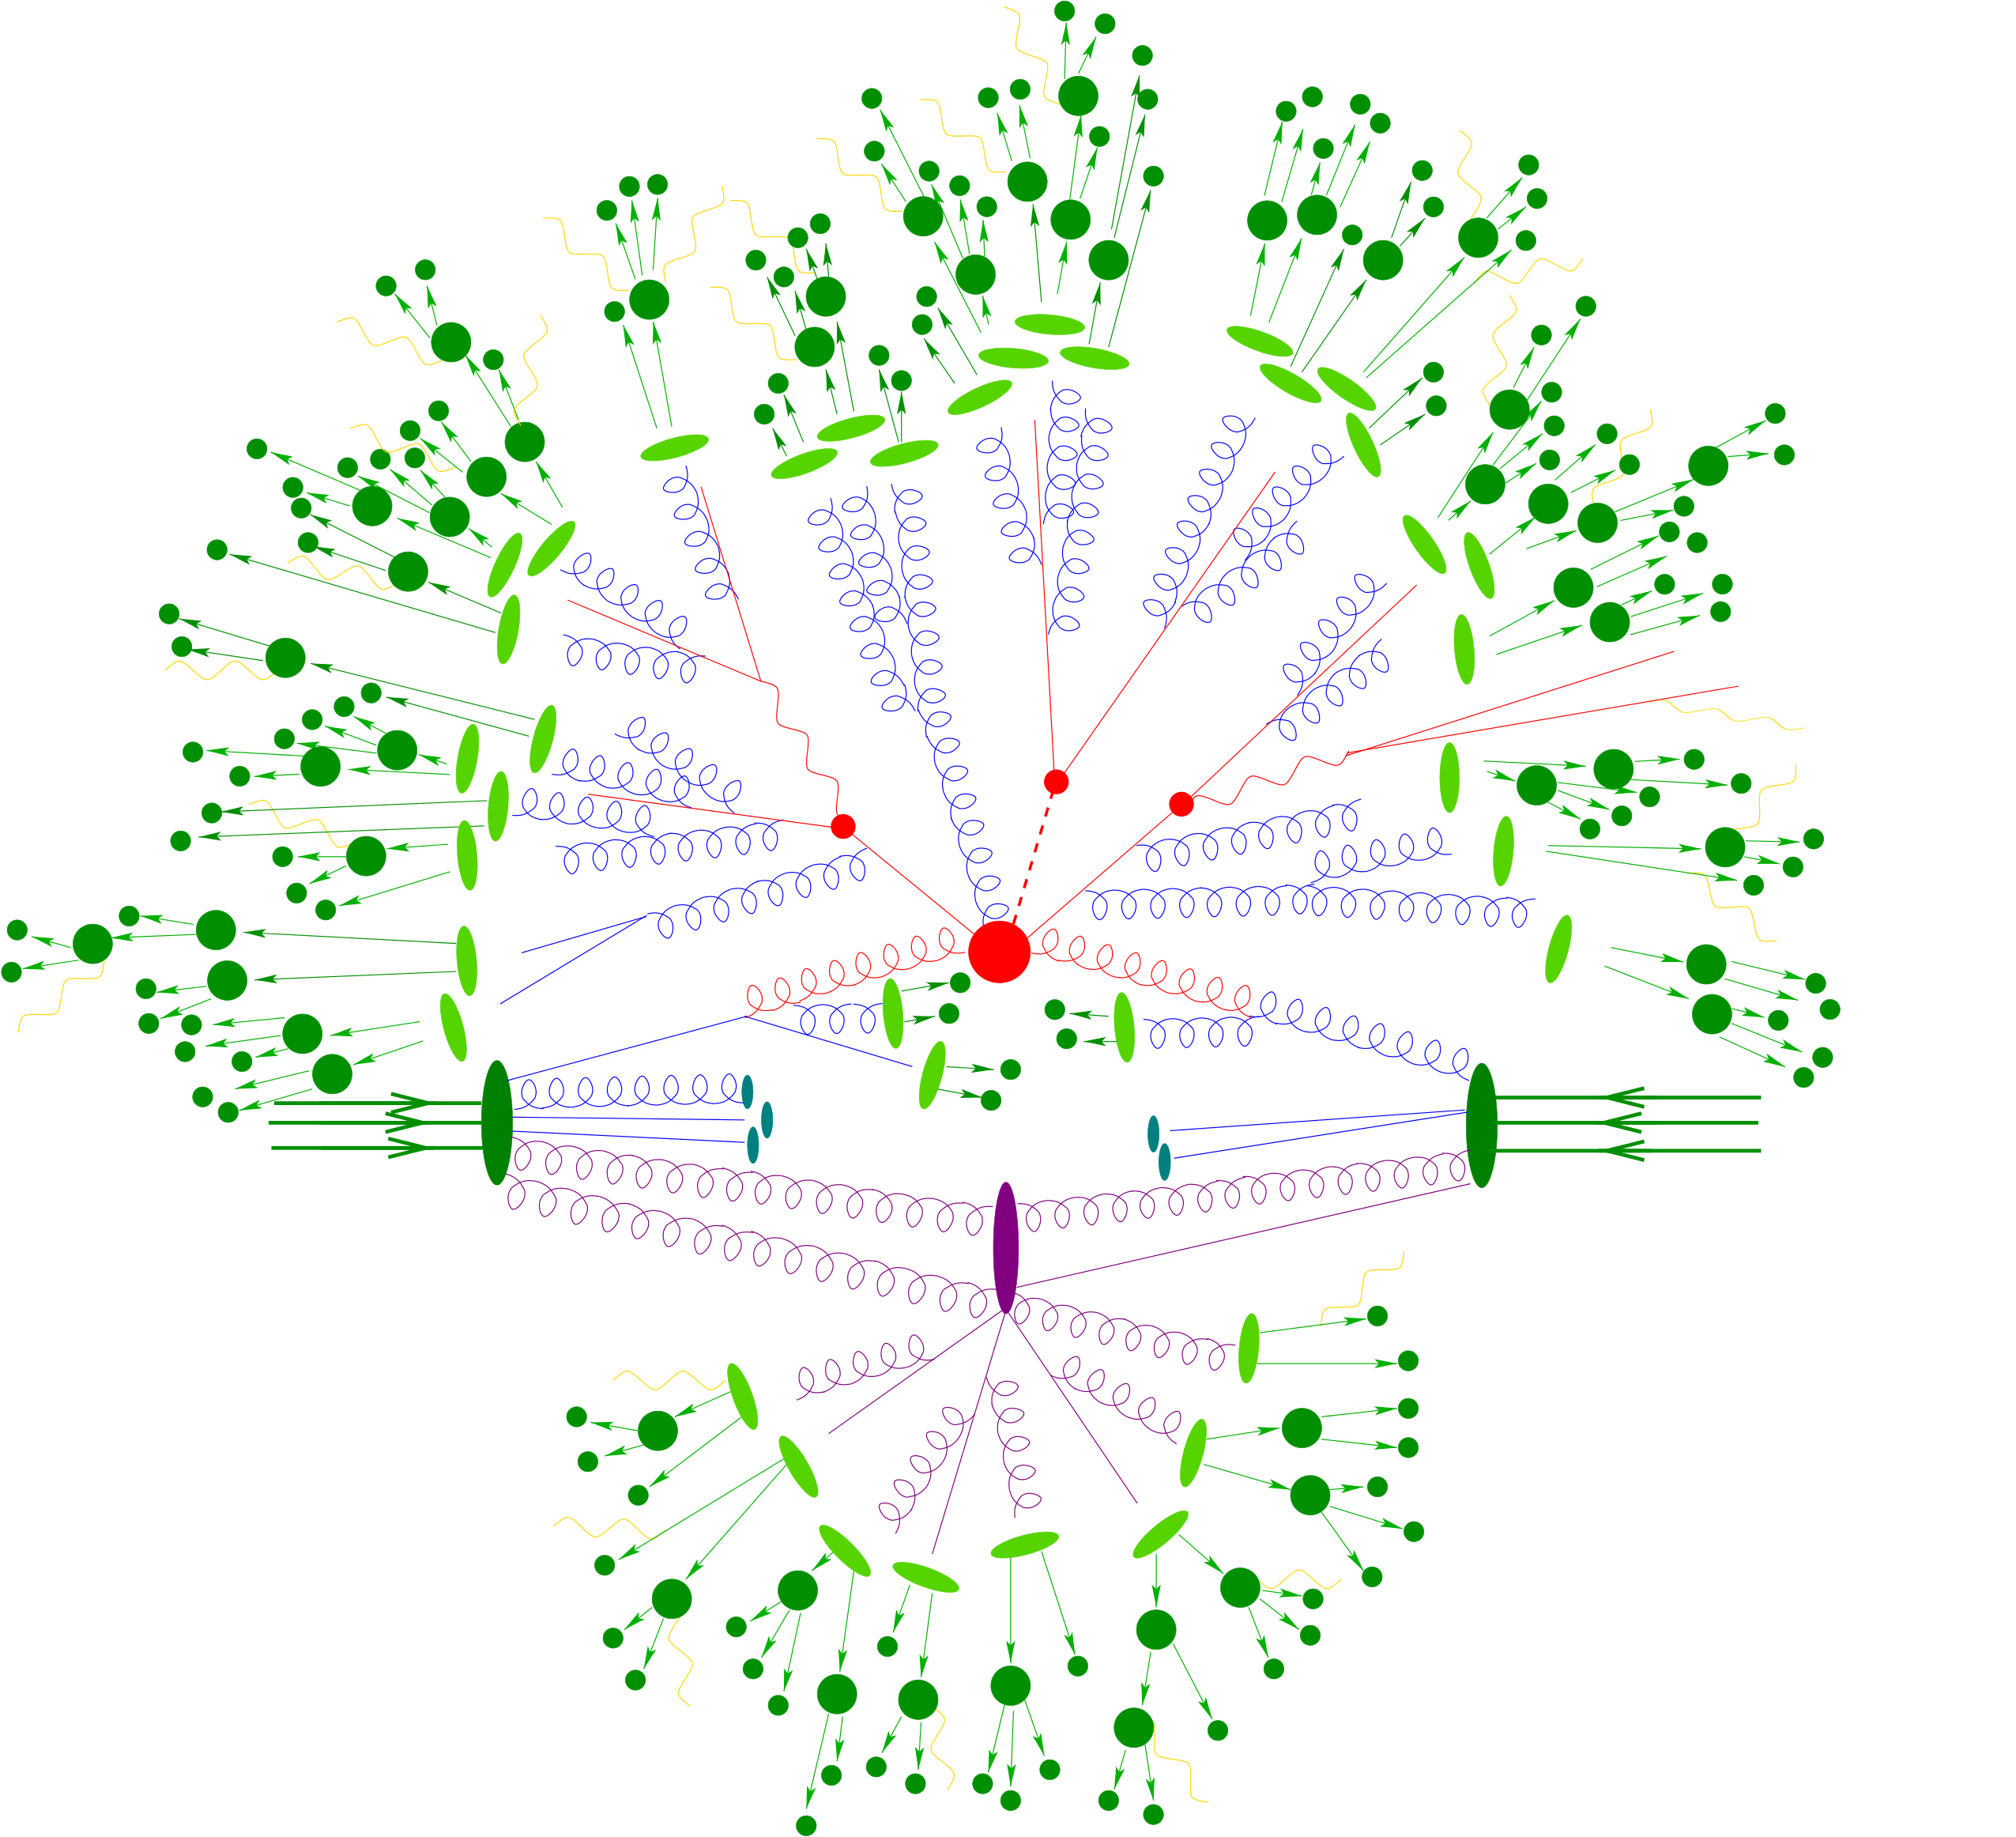
\includegraphics[width=0.5\textwidth]{MC/tth_Event}
\end{center}
\caption{Schematic view of a $t\bar{t}H$ event produced in a pp-collision: the hard scattering is shown as a red blob with the solid and dashed lines as the resulting three particles.
Independently happening multi-particle interactions are indicated by the violet blob. 
Parton showers are shown with curly lines.
Hadronization yields hadrons as shown in light green, while the final state particle are dark green.
}
\label{fig:MC_ttH}
\end{figure}

The outcome of the hard interaction could be simple scattering, their annihilation or a combination of two. In any case, the final state consist of a large multiplicity particles. The main goal of event generator is to provide a complete picture of this final states: description of the particle types and momentia on event-by-event basis. The factorisation theorem allows to make event generation in independent stages, which are dominated by different dynamics:
\begin{description}

\item[Modelling of hard subprocess] Hard subprocess is happening at the smallest scales of times and distance, where all of the colliding partons are considered free and their initial momentia are given by selected PDF set. Process of interest is simulated by selecting production channels and calculating corresponding matrix elements (ME) in the desired level of accuracy in pertrubation theory . Most of the generators have leading order or next to leading order ME in $\alpha_s$. Scale of $\alpha_s$ is can be determined through renormalisation of factorisation. Also, inclusion of higher-order correction reduces scale dependency, however it makes calculations technically more difficult.
\item[Parton showering] Quarks and gluons from hard process can QCD radiation, resulting on the dozens of additional partons associated with the event. This process calculated as step-by-step evolution of momentum transfer scales from highest (hard subprocess), to the lowest (around 1 GeV). 
There is a possiblity of double counting between showers and hard subprocess. This can be avoided using matching approach, for which higher order corrections to ME are integrated with parton showers, or merging strategy, there jet resolution scale is used as an threshold between matrix elements and parton showers. 
\item[Hadronisation] Final stable color-neutral particles, what can be detected in experiment, are formed during hadronisation. This occures at larger nonpertrubative scales and  usually implemented using different phenomenological models.
\item[Modelling underlying event] Parallel to the main process other collisions of partons can occur, called underlying event. These additional interaction can produce partons which contribute to the final state. This is one of the least understood aspect of hadronic collisions. 

\end{description}

Schematic plan of simulation of ttbar event is shown on a figure \ref{fig:MC_ttH}. The hard scattering itself is shown as a red blob with the solid and dashed lines indicating the resulting particles, which themselves decay further. 
Underlying event is indicated by the violet blob. 
Parton showers are shown with curly lines.
Hadronization yields hadrons as shown in light green, while the final state particles are dark green.

The current analysis uses samples generated with the following generators:
\begin{itemize}[align=left]
\item[Powheg]Powheg is generator with NLO ME, that can be interfaced with other generator(such as Pythia or Herwig) for higher precision of showering.
\item[Pythia] Pythia is a general purpose generator for hadronic, hadron-lepton and leptonic collisions. It can model initial and final state showers, hadronisation and decays, underlying event (via multi parton interactions). Pythia contains library with around 240 processes with LO ME. It uses Lund String model for hadronisation.
\item[Herwig] Herwig is a LO general purpose event generator for simulation lepton-lepton, hadron-lepton and hadron-hadron collisitons. The main difference between Pythia and Herwig is that it is uses angular ordering in the parton showers and also models the hadronisation step based on the cluster fragmentation
\item[Sherpa] Sherpa is a generator with tree level of matrix elements, featuring its own implementation of parton shower and hadronisation models.
\item[Photos] Precision tool for QED radiative corrections in W and Z decays.
\item[Tauola] Generator, used to describe leptonic ans semi-leptonic $\tau$-decays.
\end{itemize}

\subsection{Simulation in Geant4}

After event generation, simulation software obtains hardware response for a final state particles. The main method used by ATLAS, referred to as \textit{Full Simulation}, makes use of the Geant4\cite{Geant4}. It is C++ based toolkit for the simulation of the passage of particles through matter. It is used in a wide range of experiments in a high energy, nuclear, medical and space experiments.

Geant4 can simulate complex detector structure with sensitive detector material and corresponding infrastructure. It can also calculate basic properties of materials, like radiation and interaction length. For detector Geant4 stores "hits" information  - snapshots of physical interactions. 
In Geant4 events are simulated separatelly and each particle is moved step by step. Size of this step is chosen to preserve both CPU performance and required precision. Physics processes are handled either at rest, along step or after. Geant4 package has different models and approximations of hadronic and electromagnetic processes. Some of them are not so precise, but computationally fast. It allows to choose set of the models, called physics list, depending on a case. There are several reference physics lists, that are validated for each new release. ATLAS experiment is using one of this lists.

It is necessary to have a mass MC production for each data taking, what is taking most of the resources.  Some of the Run-1 analysis are dominated by available MC statistics. 
It is possible to improve in CPU usage by tuning physics list or reworking of B-field access. Also there are long term developments for multi-threading and vectorisation of the code. 
Yet, Run-2 has a higher pileup and luminosity, so even more MC events are needed. This means that fast and accurate simulation approach is essential. During simulation largest time is spend on calorimeters. This is the motivation for development of fast calorimetry techniques.  
There are two main methods used in ATLAS:
\begin{itemize}
\item Parametrisation of calorimeter cells responce. Spacial energy responce is simulated using longitudial and lateral energy profiles.
\item Frozen Showers. This technique will be described more detailed in the following section
\end{itemize}


\subsection{Frozen Showers}
Main principle of this library is described by it's name. It is using pre-simulated "frozen" showers generated in a full simulation. Particles below minimum energy
thresholds are killed and replaced with with this showers. All of the other particles are using full simulation. This process is schematically shown on a Figure ~\ref{fig:MC_FS_method}.
\begin{figure}
\center{
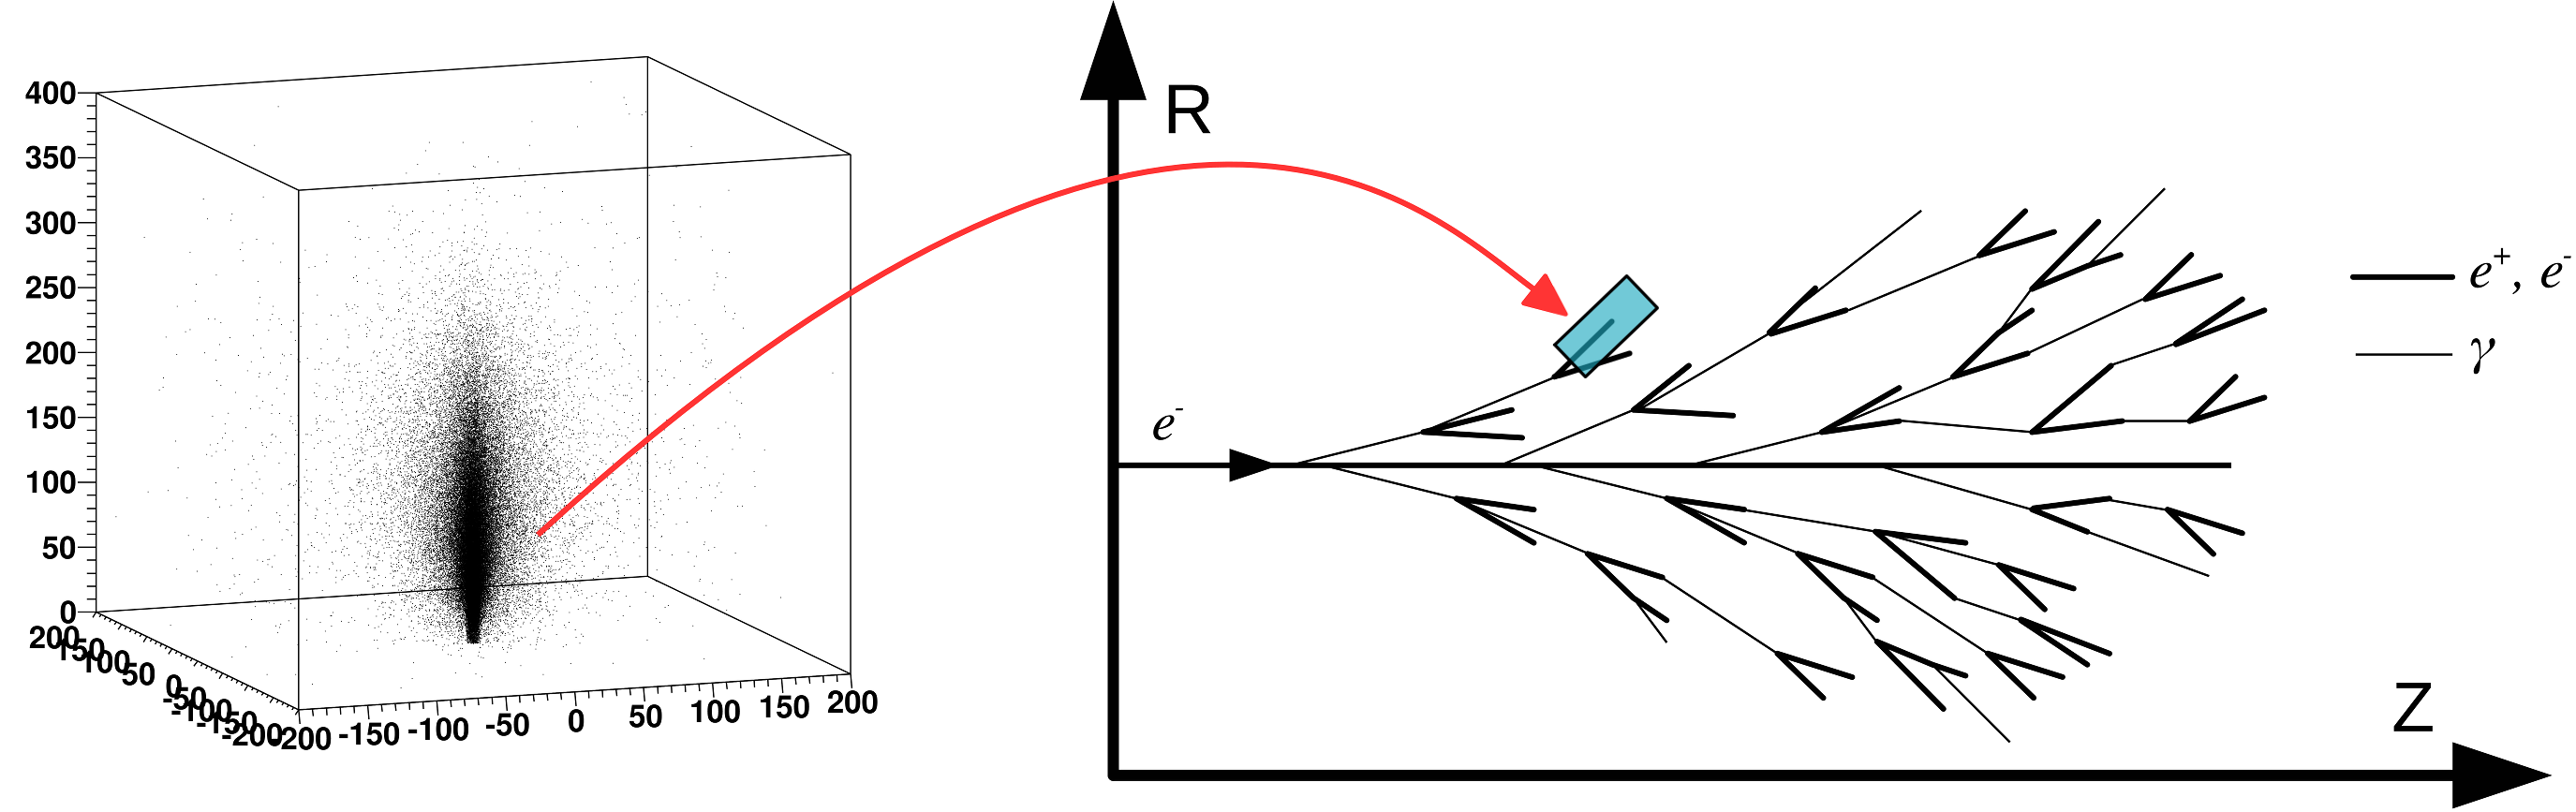
\includegraphics[width=1.0\textwidth]{MC/MC_FS_method.png}
\caption{Diagram showing the shower substitution of the low-energy particle, during the high-energy particle simulation.}
\label{fig:MC_FS_method}}
\end{figure}
The library itself organized as follows: it contains basic simulation parameters, like Geant4, geometry and atlas software release version and physics list used. It stores information about position of initial particle in a bins, energy remains unbinned. For showers it has list of hits, that are containing four vector (time and position) and energy deposition. There is also additional information about lateral and transverse size of the shower. 

\subsubsection{Production use of Frozen Showers}

\begin{figure}[h]
\begin{minipage}[h]{0.49\linewidth}
\center{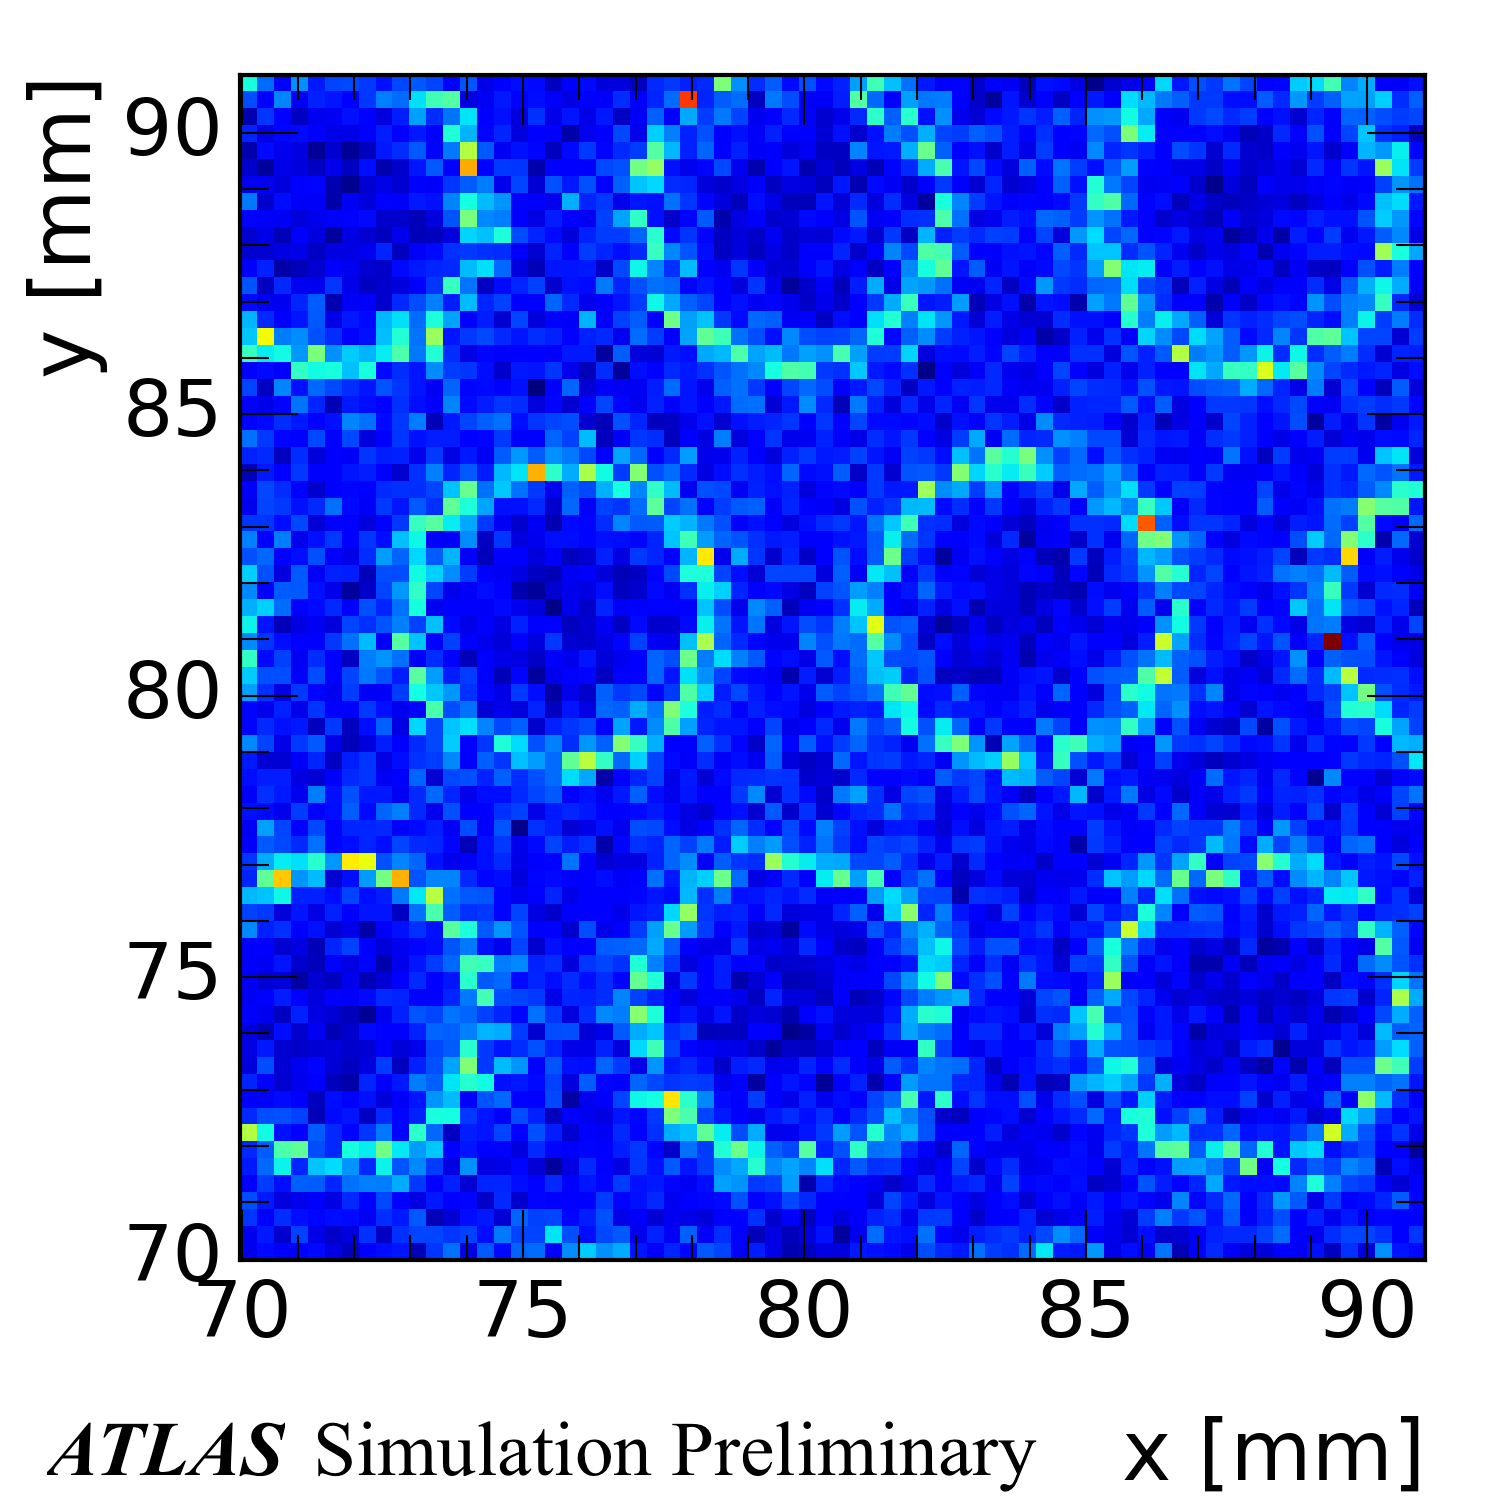
\includegraphics[width=1.\linewidth]{MC/xySumE.png} \\ a)}
\end{minipage}
\hfill
\begin{minipage}[h]{0.49\linewidth}
\center{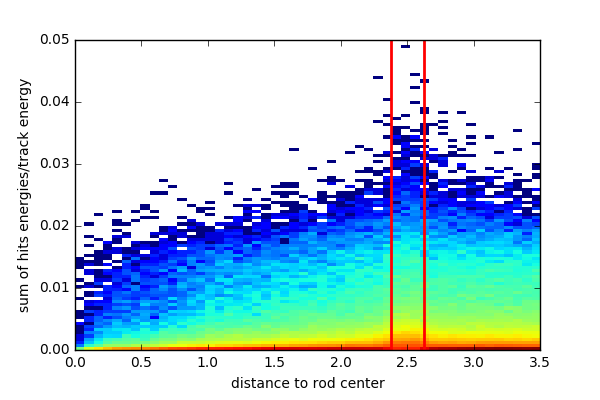
\includegraphics[width=1.\linewidth]{MC/fullBinningScatter.png} \\ b)}
\end{minipage}
\vfill
\begin{minipage}[h]{0.49\linewidth}
\center{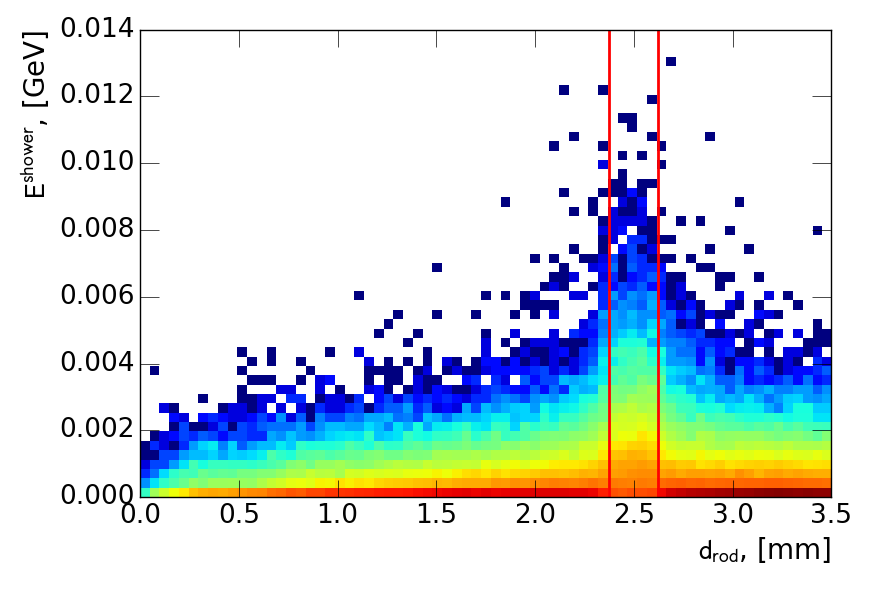
\includegraphics[width=1.\linewidth]{MC/fullBinningScatterSmall.png} \\ c)}
\end{minipage}
\hfill
\begin{minipage}[h]{0.49\linewidth}
\center{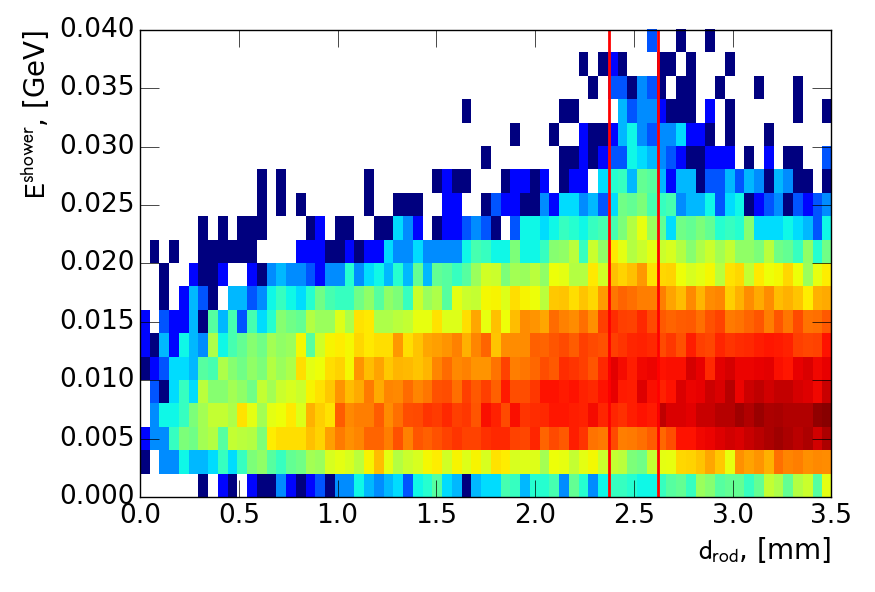
\includegraphics[width=1.\linewidth]{MC/fullBinningScatterBig.png} \\ d)}
\end{minipage}
\caption{Energy responce for electrons in a calorimeter a)in a x vs y plane and  in a distance plane  for b) all electrons in a libary  c) electrons with energy less than 100 MeV d) electrons with energy bigger, than 100 MeV}
\label{fig:Class}
\end{figure}


During a simulation, if an energy of particle falls below cut-off energy, particle is stopped and killed and substituted by shower from library. Also, it is checked, that particles is far away from the edges of calorimeter, so what resulting shower will be by 90\% contained in a calorimeter. This check is energy dependent, since shower sizes are growing with the energy. 
When particle is removed, it is substituted by shower taken from corresponding eta and distance bin with the closest energy found. Energy of the hits in shower is scaled to fully correspond to particle energy. Also, shower direction is changed to the direction of the shower.

Frozen Showers have been used in Atlas Monte-Carlo production since run-1. This method is applicable for all LAr calorimeters in ATLAS, but currently it is enabled for simulation of forward calorimeters (FCAL), since it is showing the smallest differences, compared to the other fast simulation methods (e.g parametrisation). This is happening because of large of non-uniformly distributed sensitive material (citation to previous chapter). Energy resolution of calorimeter on a fixed energy depends only on a two statistical factors: fluctuations of the energy loss and number of produced charged particles. Additional binning variables are allowing to capture this non-uniformities. Example of this is in picture .... Sum of the deposited in a sensitive material "hits" divided by initial particle energy is shown on picture. Gap position is shown by the red lines. It is clear, that showers, what have been born inside sensitive material tend to have higher energy response (SumE/E) and thicker tails, than showers in a dead material. This is causing larger constant term. Introducing additional spacial binning, that is defined as distance to the closest rod center is allowing to capture this fluctuations. It can be also shown, that size of this fluctuation is depending on initial particle energy (pic. ). For electrons with energy greater than 500 GeV they are almost negligible. This is why upper limit for frozen showers was set to 1000 MeV.
This method is allowing to capture well shower-shape variables, that are later used for identification of the forward electrons. 
\begin{figure}
\center{
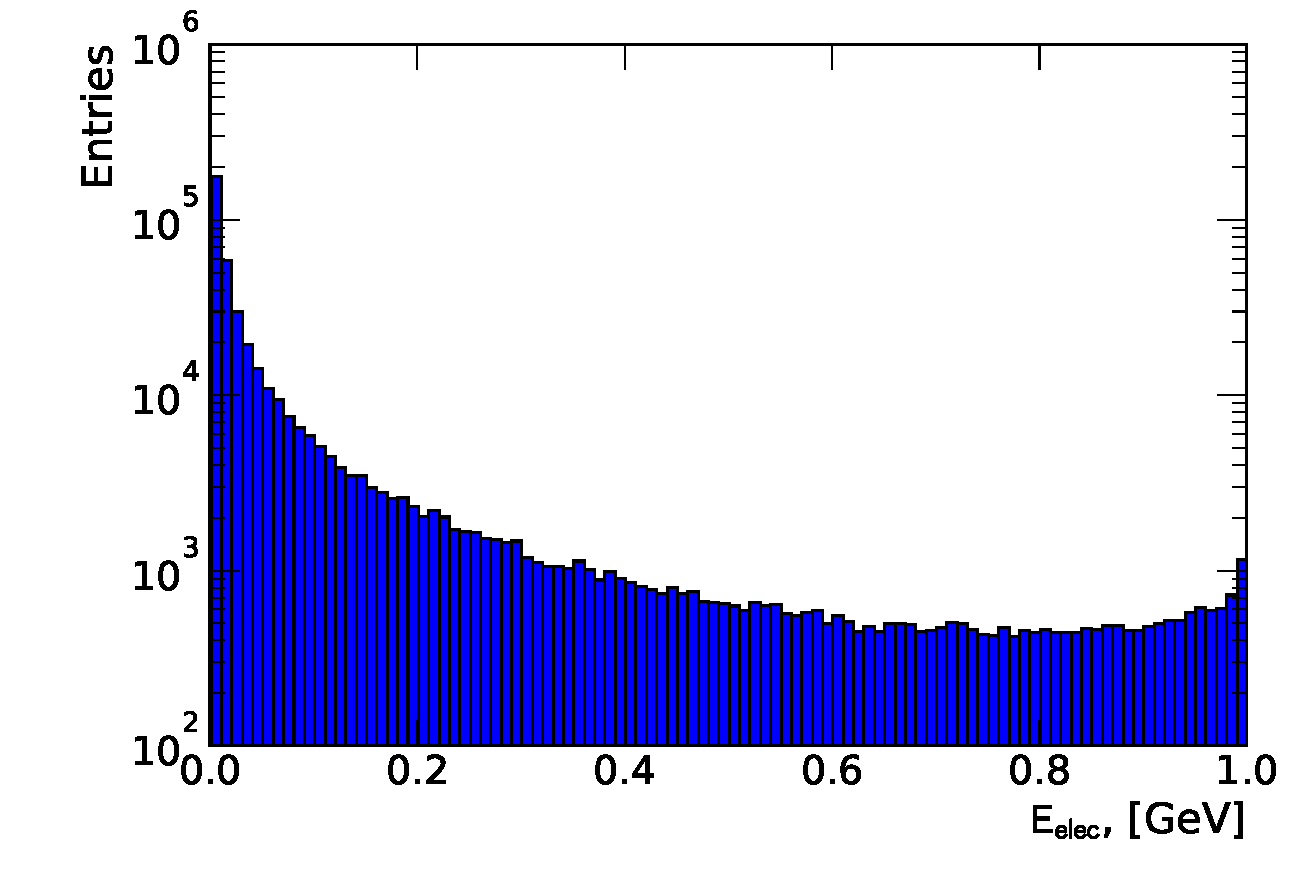
\includegraphics[width=0.8\textwidth]{MC/FSEnergy.pdf}
\caption{Distribution of shower energy used in production of 1000 GeV electrons.}
\label{fig:FSEnergy}}
\end{figure}
Distribution of shower energies, used for production of high-energetic electron (1000 GeV in that case), is shown on a Figure ~. More than 50\% of them are having energy less than 20 MeV. Studies have showed, that Frozen showers are slower, than a standard Geant4 simulation for showers with energy 3 MeV. This is happening due to library non-binned structure for energy. This makes search of closest energy shower in a library slower, than simulation of shower with zero or one hit in a sensitive detector. 

\subsubsection{Generation of Frozen Showers library}

\begin{table}
\centering
\begin{tabular}{l|r}
\hline
\hline
\multicolumn{2}{c}{The general frozen showers parameters} \\
\hline
Detectors used            & FCAL1, FCAL2, FCAL3 \\
Type of the particle      & photons, electrons, neutrons \\
Energy range              &  $E_{\gamma}<10$~MeV,  $E_{e}<1000$~MeV,  $T_n<100$~MeV \\
Containment requirement   & $\Delta E_{shower} > 98\%$\\
\hline
\multicolumn{2}{c}{The library post-processing parameters} \\
\hline
Generation clustering cutoff & $(\Delta R_{cluster})^{2} < 25$ mm\\
Generation truncation cutoff & $R_{hit}^{2} < 50000$ mm, $\Delta E_{shower} < 1\%$\\
\hline
\hline
\end{tabular}
\caption{Main parameters used for the frozen shower libraries in FCAL }
\label{tab:MC_FS_params}
\end{table}

In a Frozen Shower method there are separate libraries for each particle and subdetector used. Showers should cover fully energy and pseudorapidity region and be able to describe data, that is needed during simulation. This is why 2 stages simulation approach have been used. The first stage is to take initial particle parameters, that later will be used in a library from a physical process. This is done using simulation of some process (e.g. ttbar or single electron). Every time, when particle becomes eglighable for Frozen Showers, it is saved as a starting point. Particles are tend to clustere tightly around original track, so in order to achieve a better detector coverage on a smaller sample, this primary points are randomly truncated. On the second stage, simulation for this primary vertexes is performed, using standart Atlas simulation infrastructure. This is allowing to take into account sampling fluctuations and charge-collection effects on a hit information automatically. Furthermore, in order to save disc space as well as a memory consumption, hit information is compressed. This compression is done in a two steps, hit merging and truncation:
\begin{itemize}
\item if the distance between any two hits is smaller, than a given parameter $R_{min}$, then hits are merged into one deposit at the energy weighted center of them. This process is done iterativelly.
\item hits whose energies are below the fraction f of the total energy sum of all hits, are truncated. The energy of remaining hits is rescaled back to preserve the total deposited energy.
\end{itemize}
Unfortunately, for a Frozen Showers, generated for Run-1 monte-carlo, additional tuning of electron libraries was needed. This was done using reconstructed energy of electrons. Frozen Showers tend to underestimate fluctuations of energy loss, that is leading to a smaller electron resolution for a high energies. Correction is done by enlarging bin, corresponding to a gap position. Also, correction of the mean shift is done by scaling energy response of all showers. After this frozen showers are showing good agreement with full simulation. This procedure needs to be done every time, when something is changing in software. Because tuning is done manually, lots of a manpower is needed for each Monte Carlo mass production campaign.



\begin{figure}[h]
\center{
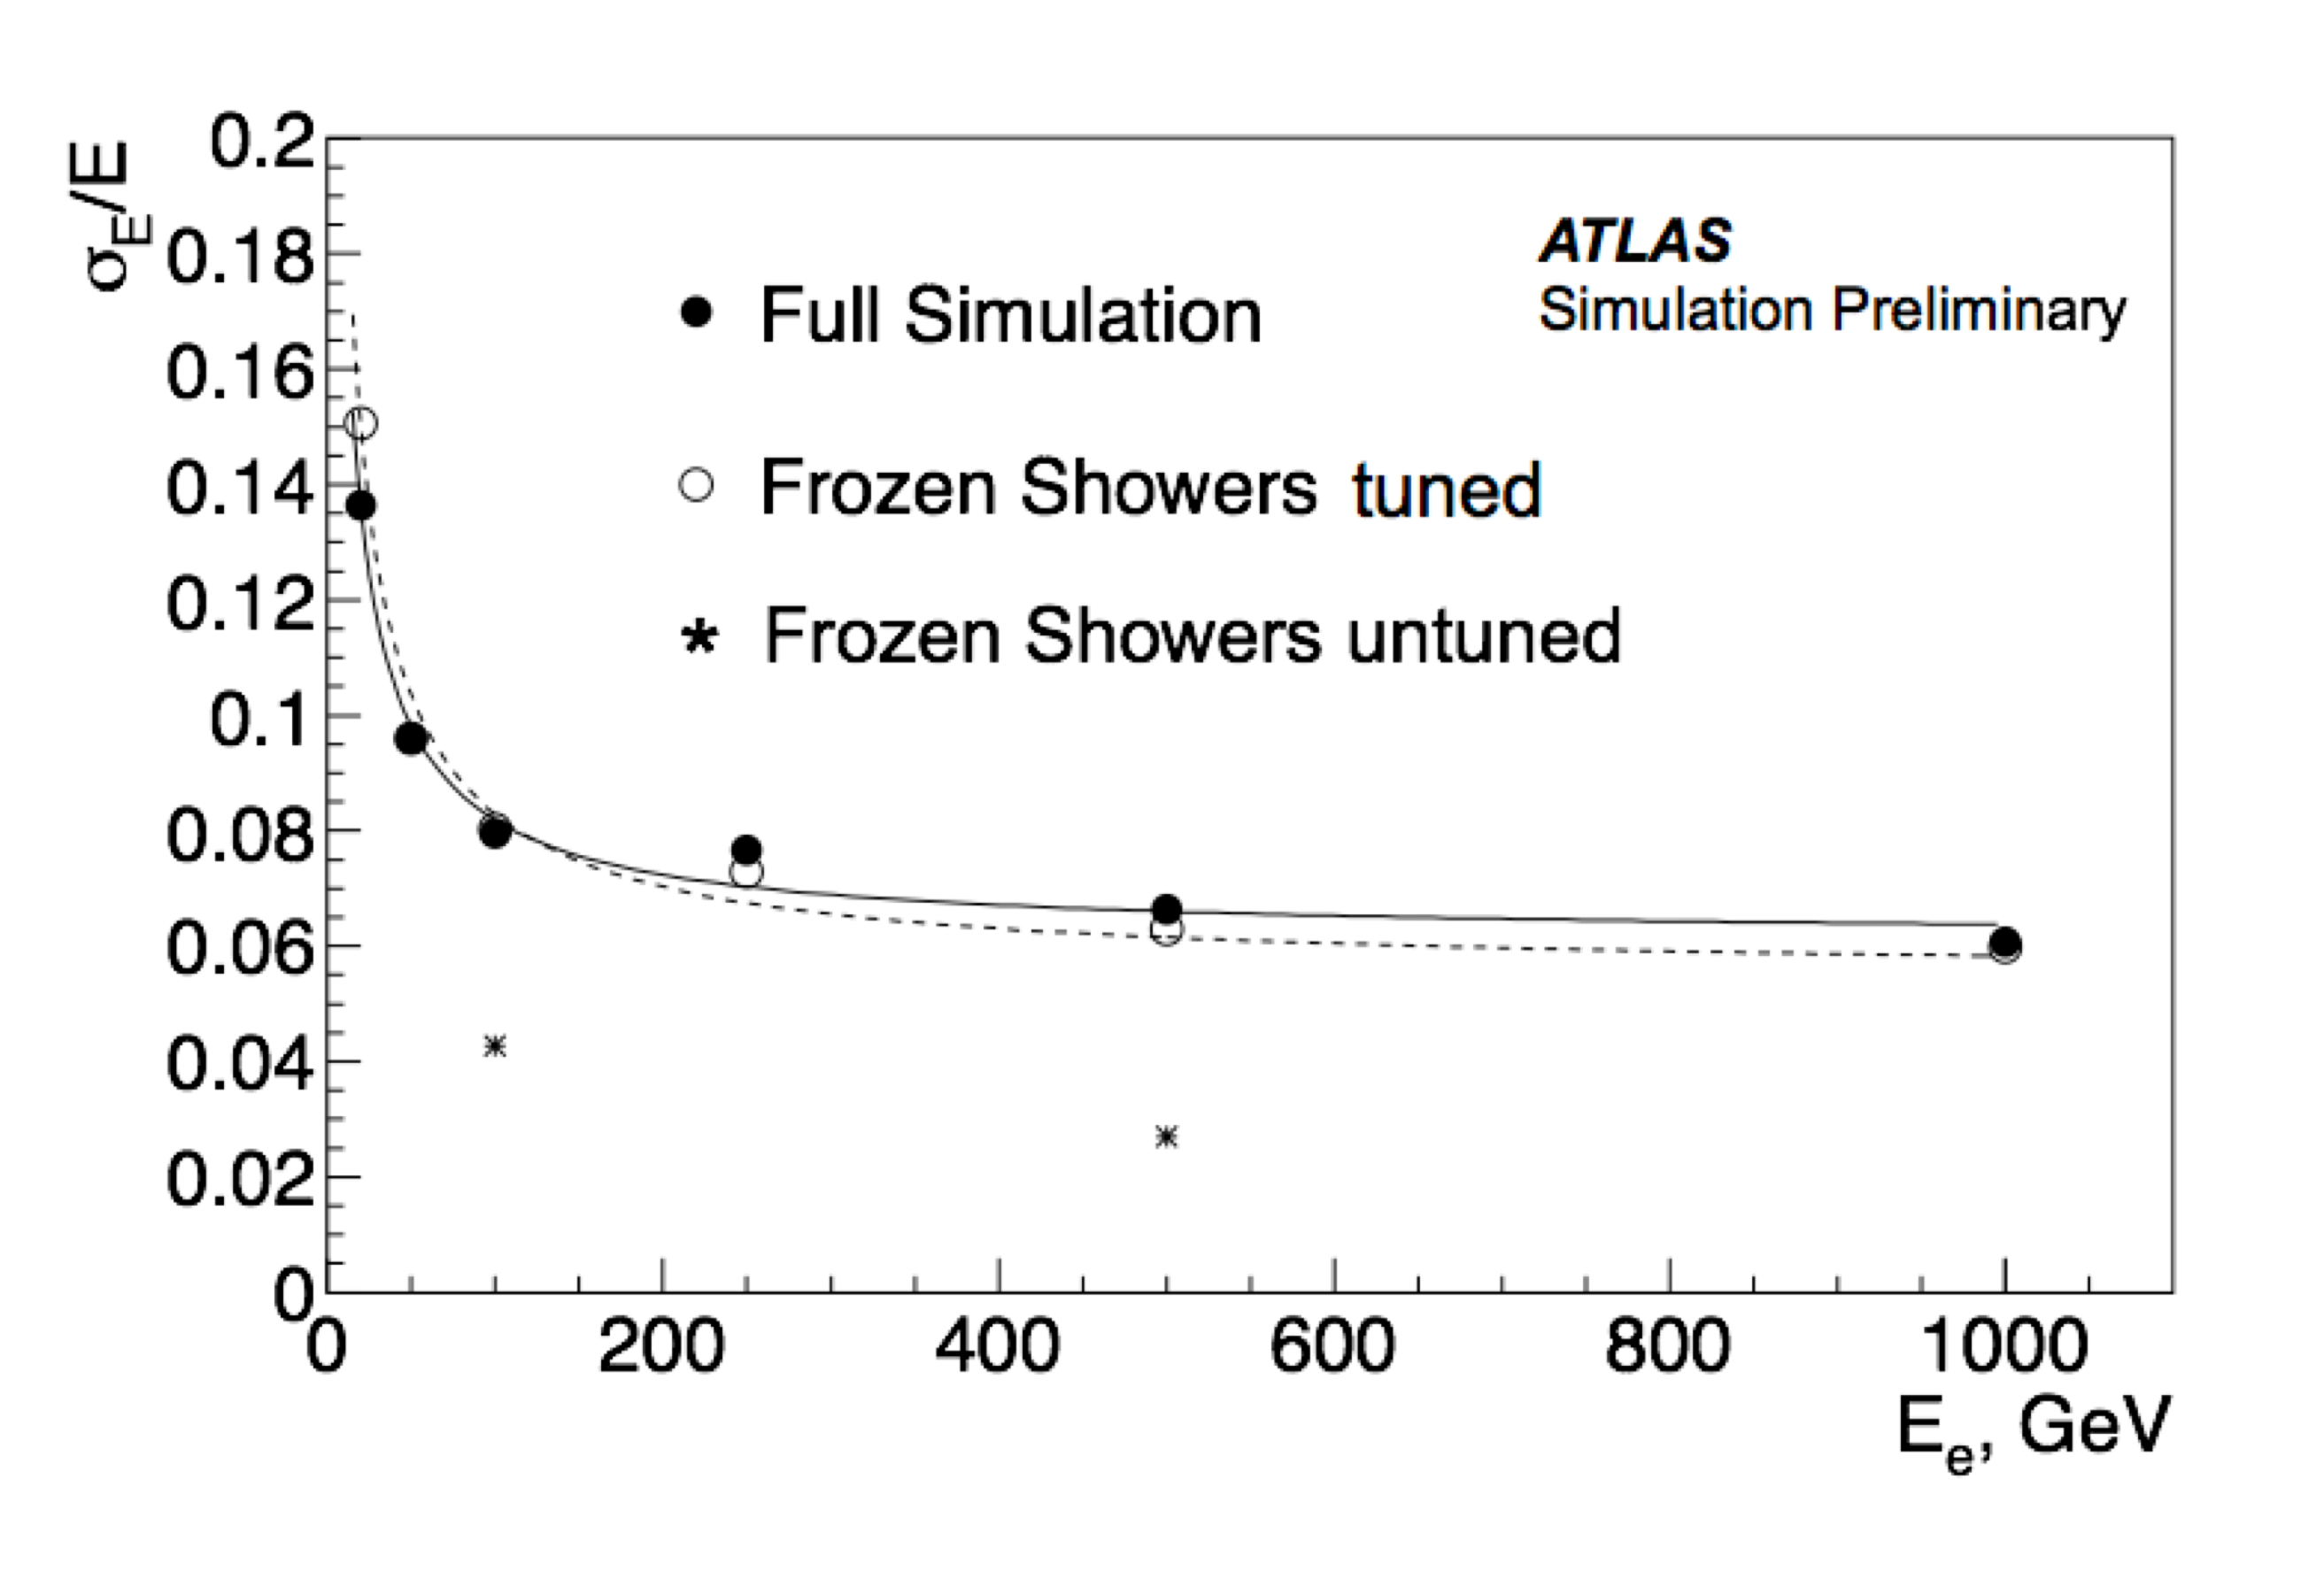
\includegraphics[width=0.7\textwidth]{MC/fs.png}
\caption{Electron resolution for full simulation, tuned and untuned frozen showers}
\label{fig:FS_resolution}}
\end{figure}

\subsubsection{Distance binning problem}
As it was mentioned before, process of library generation can be comlicated and take a lot of the time because of the needed tuning. In this subchapter possible ways to improve frozen showers performance have been studied. 
\begin{figure}
\center{
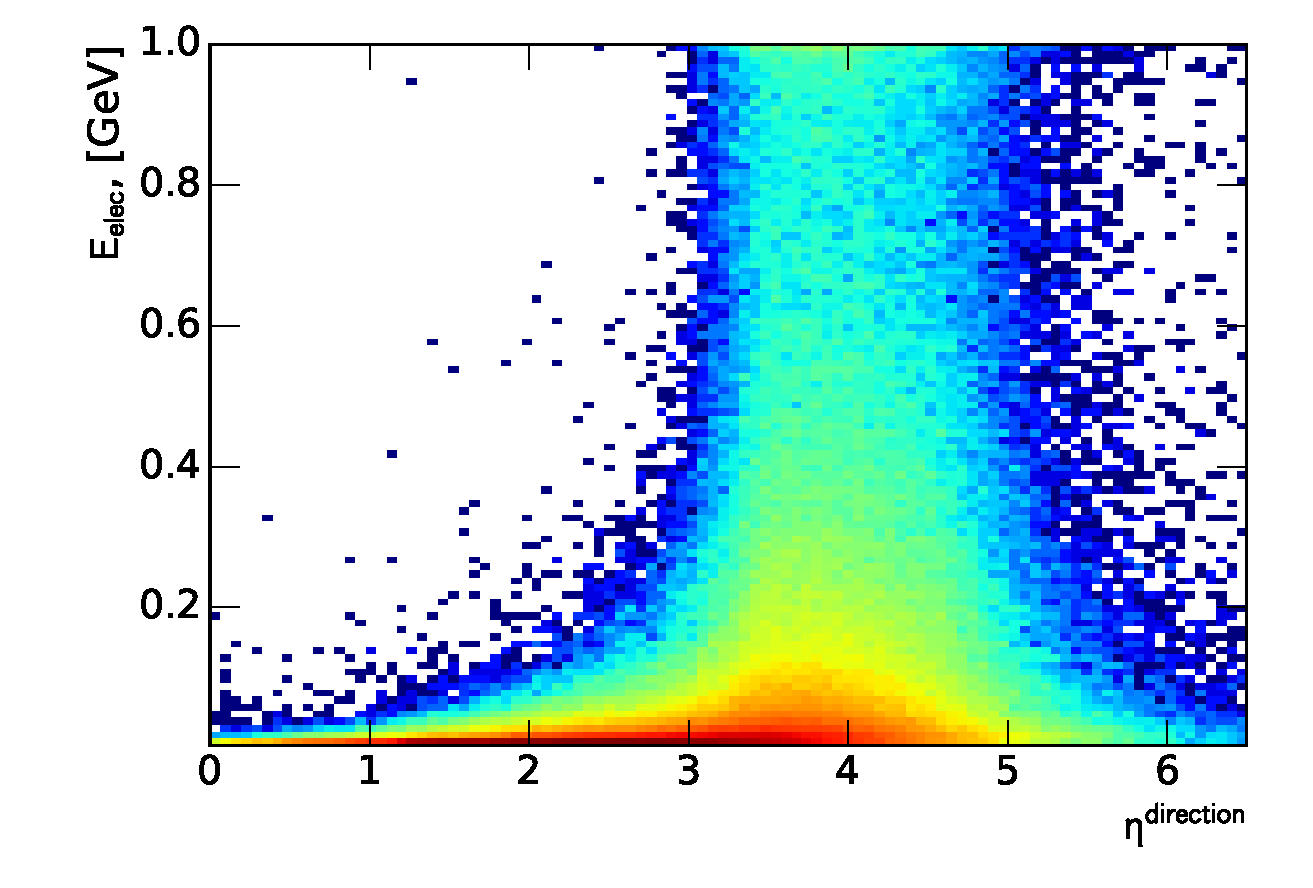
\includegraphics[width=0.8\textwidth]{MC/FSEtaMomVsEnergy.pdf}
\caption{Distribution of showers used in production of 1000 GeV electrons on shower energy vs $\eta_{momentum}$ plane.}
\label{fig:EtaMomVsEnergy}}
\end{figure}
As it was mentioned before, that there are two type of material used in a FCAL and showers within them are giving different response, what is affecting overall reconstructed electron energy resolution.  At the first generations distance bin have been corresponding to LAr gap or dead material positions. During tuning bin with LAr was enlarged to gain a better agreement with full simulation. So, one of the basic ideas to improve frozen showers performance is to change a binning, that is used during Frozen Showers library generation. It was decided to treat showers, that have been born near LAr gap and crossed it on a radiation length, in a same way with showers in sensitive material gap, and call them sensitive material showers. Oppositely, showers, that haven't crossed LAr gap, are called dead showers. This model leads to a bigger gap width by a definition. One of the possible ways to find this bin position automatically is to use machine learning tools. 

Machine Learning is a set of algorithms, what allows computers to learn and give a predictions without being specifically programmed. This is a modern field of computer science, that is wildly used in a different fields like computer vision, natural language processing, data science etc. There are two main types of machine learning algorithms: supervised, where example of desired output is given by the "teacher" and the goal is to learn a general rule, that maps inputs to outputs and unsupervised learning, then there are no labels given to algorithm, and algorithms is discovering hidden patterns in data. Initial data parameters of interest, that are used in algorithm to learn are called features. It is important to have right proper set of features and good training sample. 
From a geometrical point of view, one of the main parameter is a direction of the shower. Eta momentum distribution is showed on a Figure . Most of the showers are collinear to an electron direction. Because of this it was decided to use as a training sample simulation results for electrons with energies less than 1 GeV and momentum uniformly distributed between eta 3.0 and 4.0. This allowing to study equally low and high energy showers equally.

\begin{figure}[h]
\begin{minipage}[h]{0.49\linewidth}
\center{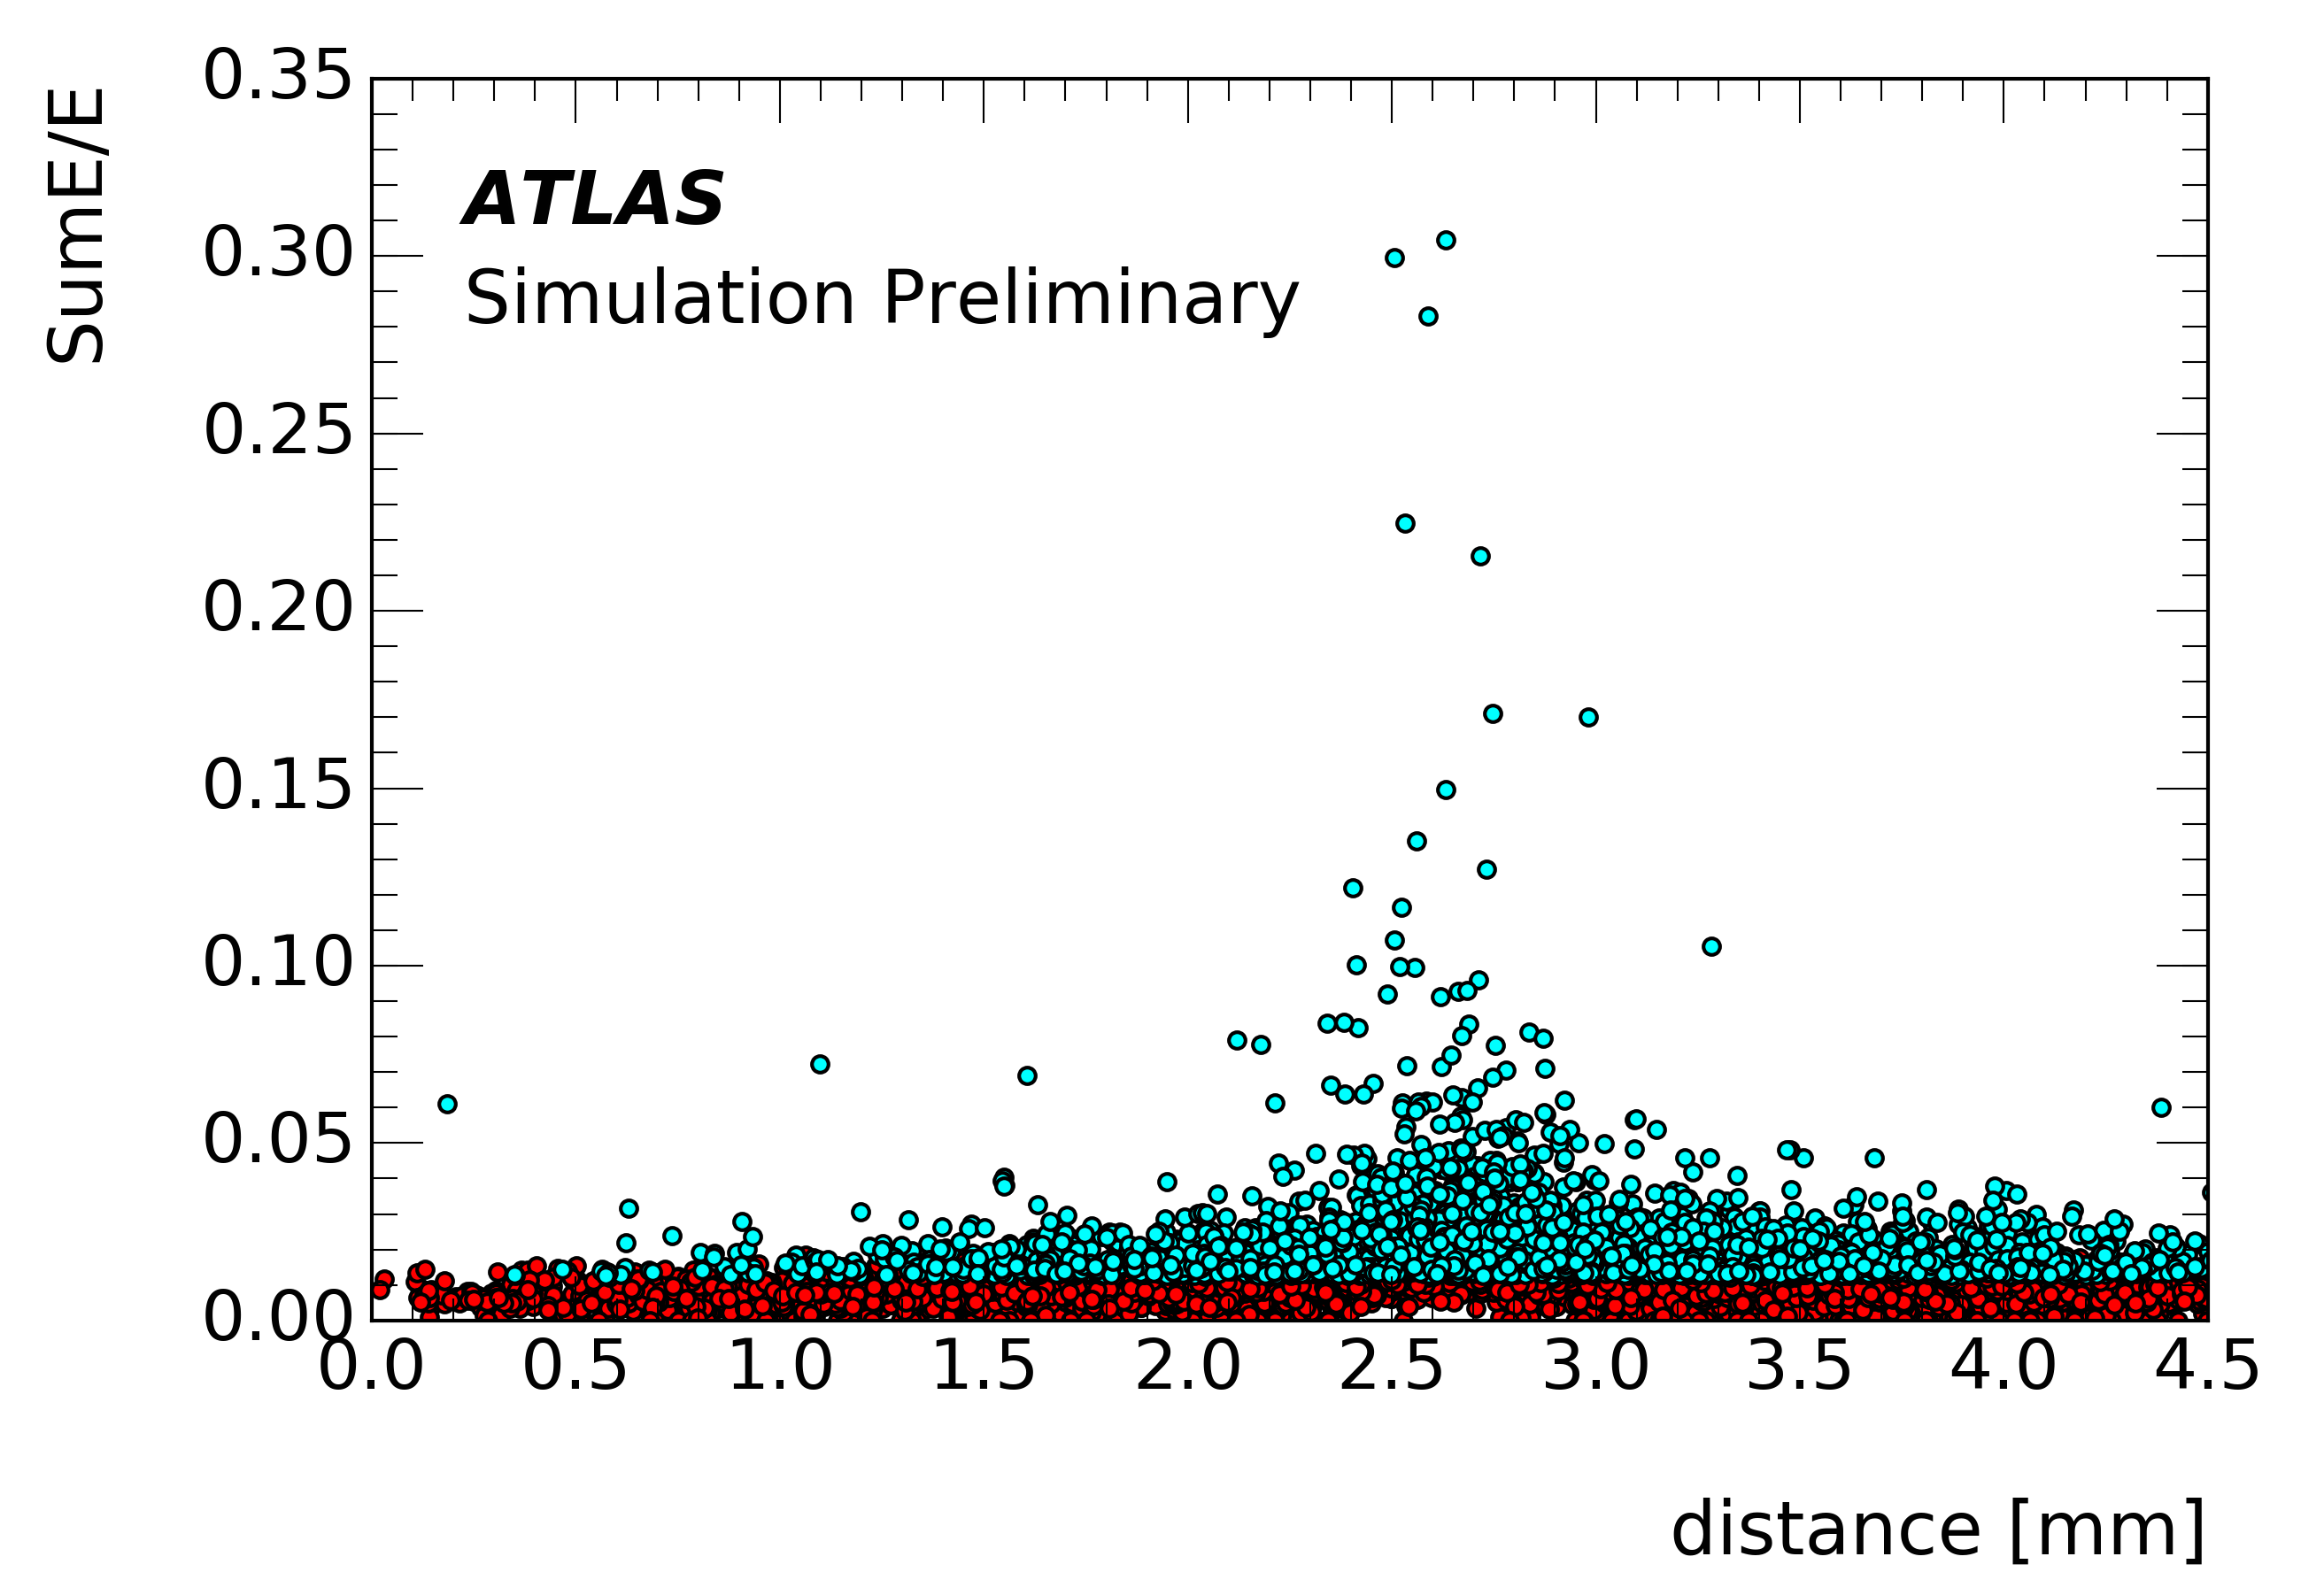
\includegraphics[width=1.\linewidth]{MC/firstClassifier.png} \\ a)}
\end{minipage}
\hfill
\begin{minipage}[h]{0.49\linewidth}
\center{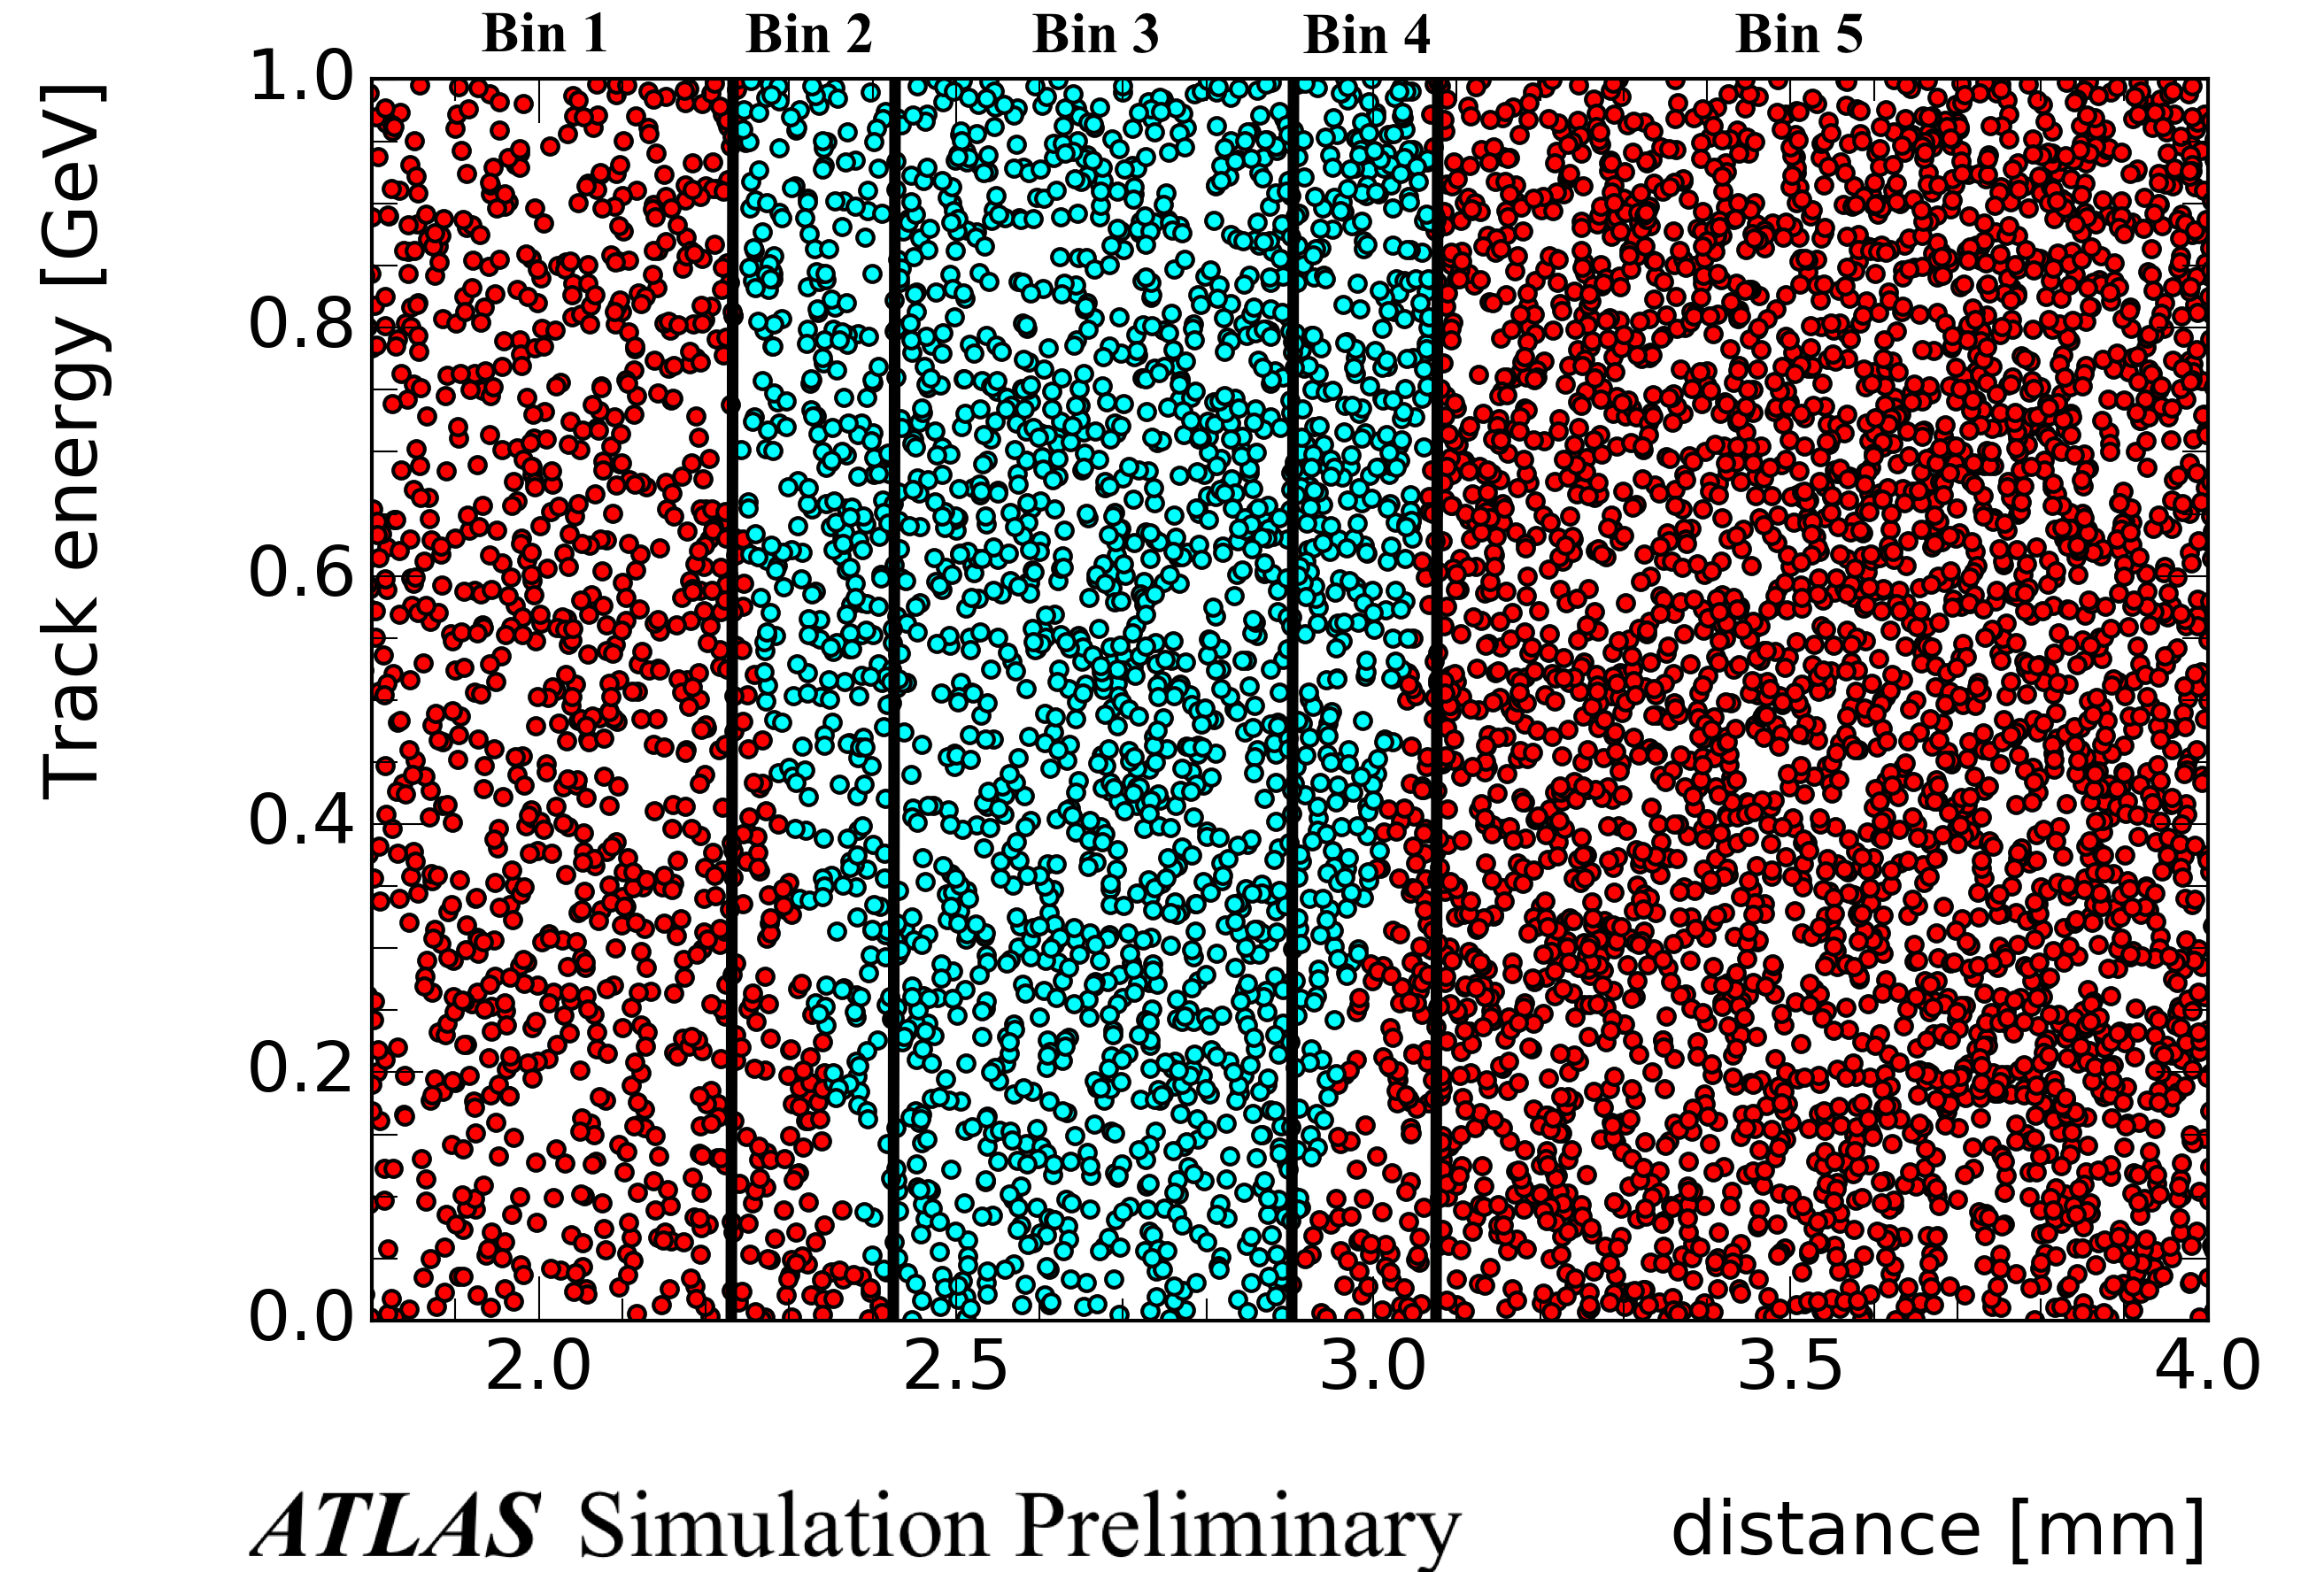
\includegraphics[width=1.\linewidth]{MC/secondClassifier.png} \\ b)}
\end{minipage}
\caption{Results of machine learning for a) first classifier b) second classifier. Cyan dots are corresponding to sensitive material showers, red - dead material showers}
\label{fig:Class}
\end{figure}


From out definition of 2 classes of showers, it is simple to construct a pre-labelled training sample. This is done by reducing initial sample and taking showers near rod center and inside liquid argon gap. Output of this classifier, that was trained on with sample with shower features, such as energy responce and number of hits, than can be used to expand our labels to a full distance range. Than it can be used as an input to a second classifier, which will separate two types of showers using particle parameters, such as energy and distance to a rod center. For a first step decision trees have showed good classification efficiency (around 97\%). For a second classifier support vector machines have been used. This method is trying to reconstruct a hyperplane, that is dividing two classes. Outputs of both of this classifiers are shown on a figure . New gap position is determined using borders of hyperplane. This procedure is giving expected from the initial model results. Gap is wider, than and original one. It is also getting bigger with bigger energy, because of the radiation length growth. 
Validation results for two different eta bins are shown on figure ~ a) and b). In a bin this new binning is performing better, than original one without any additional tuning. Unfortunatelly this is not true for all of the bins, as we can see on a figure ~ b). This eta bin have showed worst performance for a new binning, but it is performing still better, than original binning without tuning.

\begin{figure}[h]
\begin{minipage}[h]{0.49\linewidth}
\center{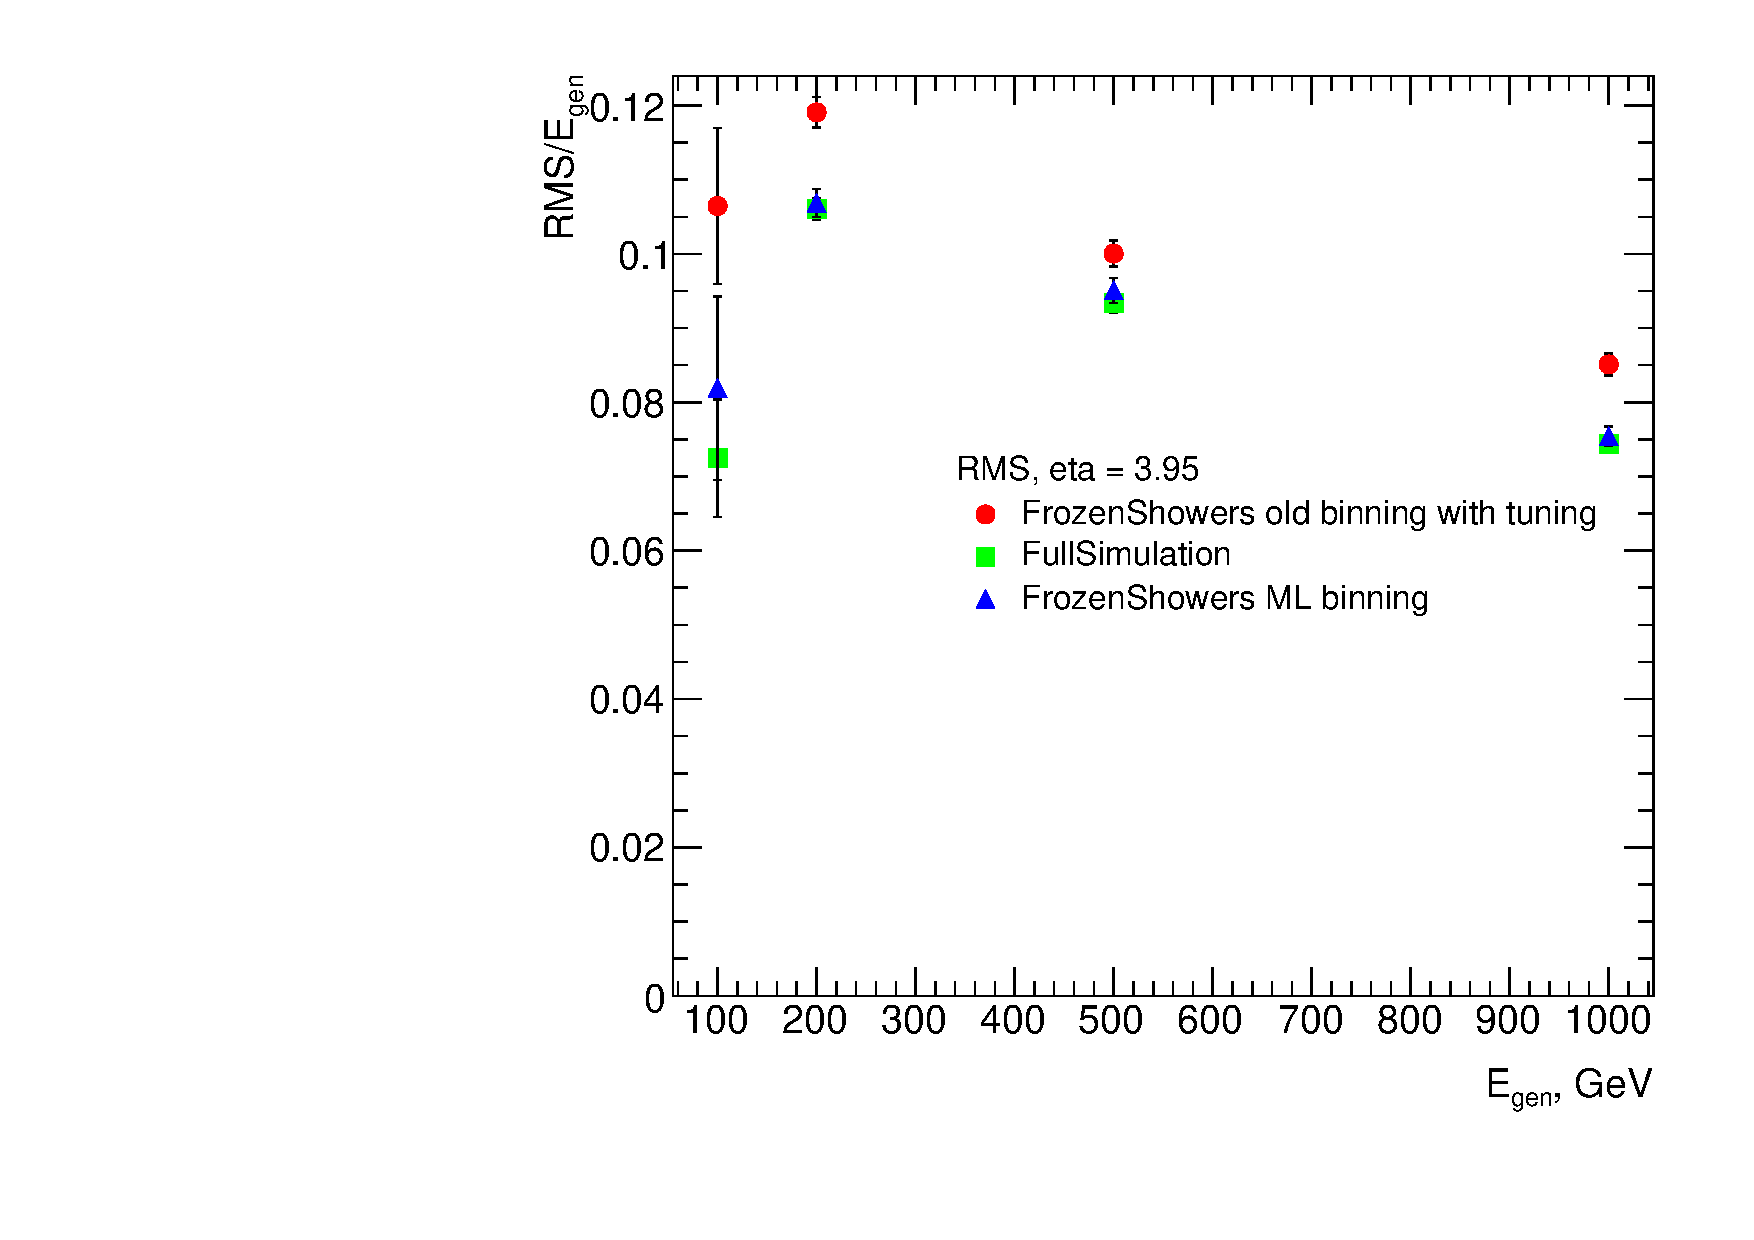
\includegraphics[width=1.\linewidth]{MC/rms3p95.pdf} \\ a)}
\end{minipage}
\hfill
\begin{minipage}[h]{0.49\linewidth}
\center{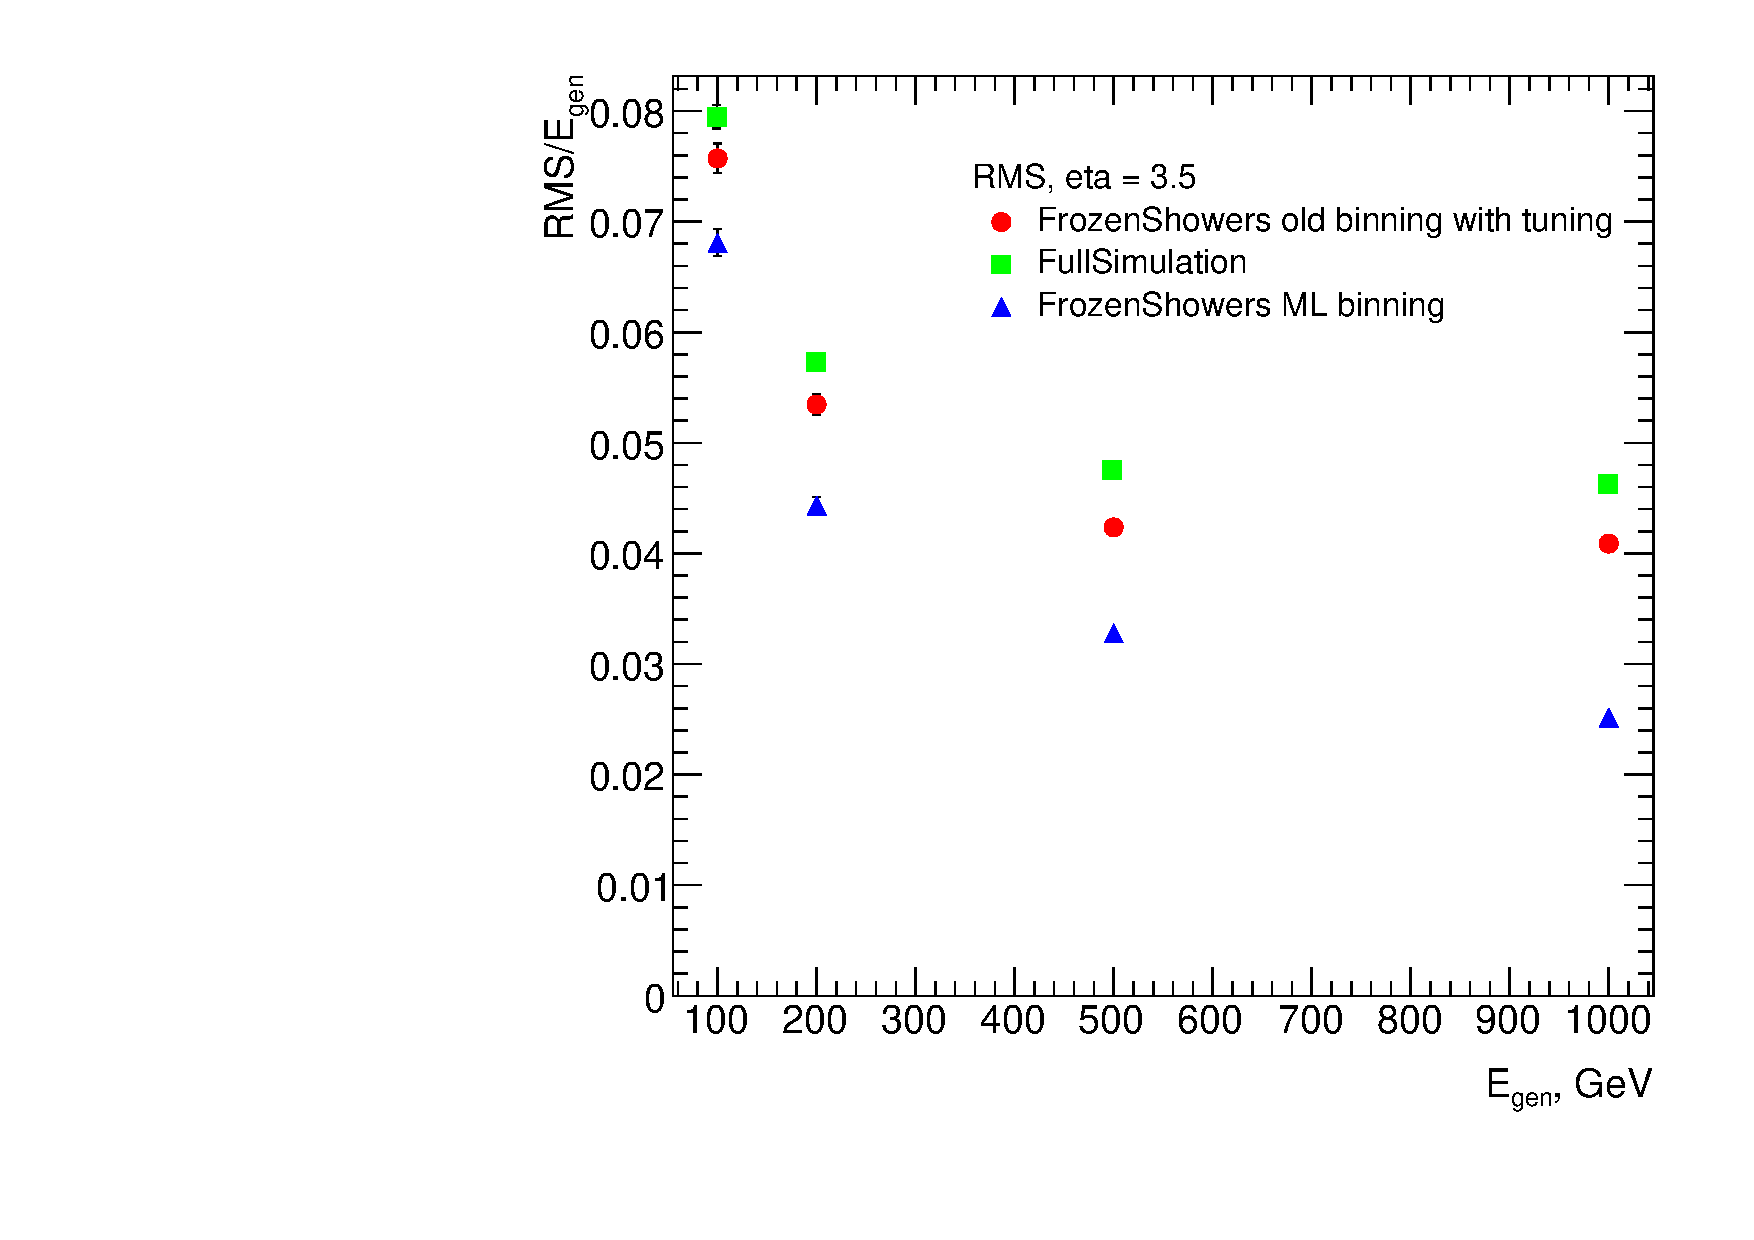
\includegraphics[width=1.\linewidth]{MC/rms3p5.pdf} \\ b)}
\end{minipage}
\caption{Resolution of reconstructed electrons for full simulation, new libraries with ML binning and old tuned libraries with original binning for a) eta =3.95 b)eta=3.5 }
\label{fig:Class}
\end{figure}

This binning was used in a production of new libraries for Monte Carlo in a Run-2. It is planned to use more precise training sample for a future iterations of this procedure for improving performance of outlying eta bins.
